\documentclass{article}
\usepackage{graphicx} 
\usepackage{hyperref}

\title{Advanced programming for HPC - Labwork 3}
\author{Son Dang Thai}
\date{October 2025}

\begin{document}

\maketitle

\section{Implementation}
\subsection{Preparation}
This labwork was carried on a 225x225 image which was imported using OpenCV
\begin{figure}[htbp]
    \centering
    
\includegraphics{rgb.jpg}
    \caption{Experiment photo}
    \label{fig:placeholder}
\end{figure}
\\This image was then flattened to 1D array of RBG before implementing the grayscale.

\section{Implementation}
\subsection{Grayscale using CPU}
By simply iterating over each row of the flattened image and setting each value equal to the average of the three values in the row, a grayscale image was produced.

\subsection{Grayscale using GPU}
Firstly, the input image and a placeholder for the output grayscale image must be fed to the kernels. Then, instead of using the for loop, each thread in the GPU must be assigned a unique index according to the flattened image to simultaneously perform the image value average algorithm. After this, the result was copied to the host to show to the user. 

\subsection{Grayscale image}
\begin{figure}[htbp]
    \centering
    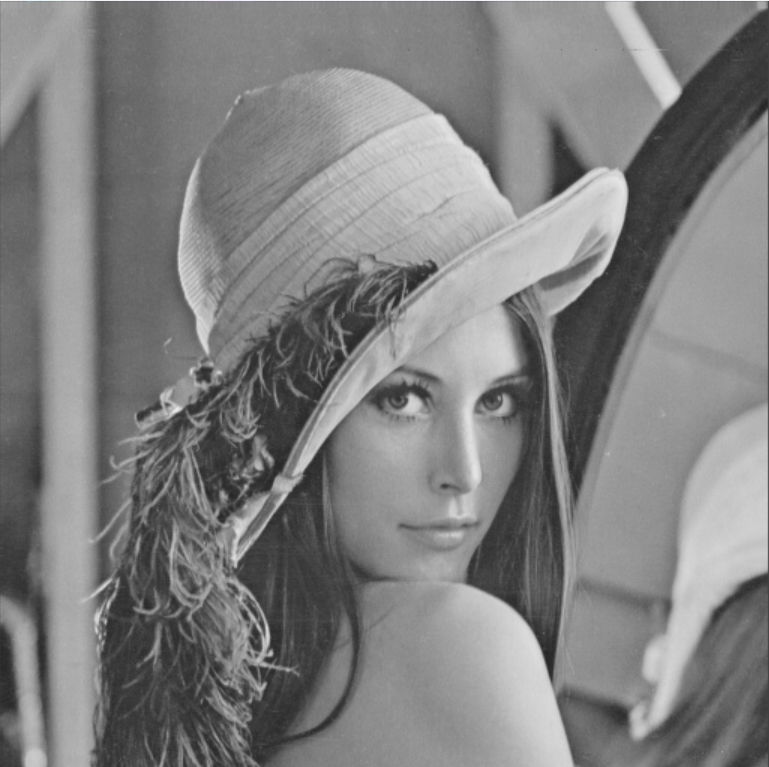
\includegraphics{grayscale.png}
    \caption{Result photo}
    \label{fig:placeholder}
\end{figure}

\section{Response time}
\subsection{CPU}
The average processing time using CPU was recorded at around 0.05 seconds.

\subsection{Grayscale using GPU}
Experimenting on different block sizes: [32, 64, 128, 256], the response time was recorded at [0.5370316505432129, 0.0001461505889892578, 8.225440979003906e-05, 6.747245788574219e-05] seconds respectively.
\begin{figure}[htbp]
    \centering
    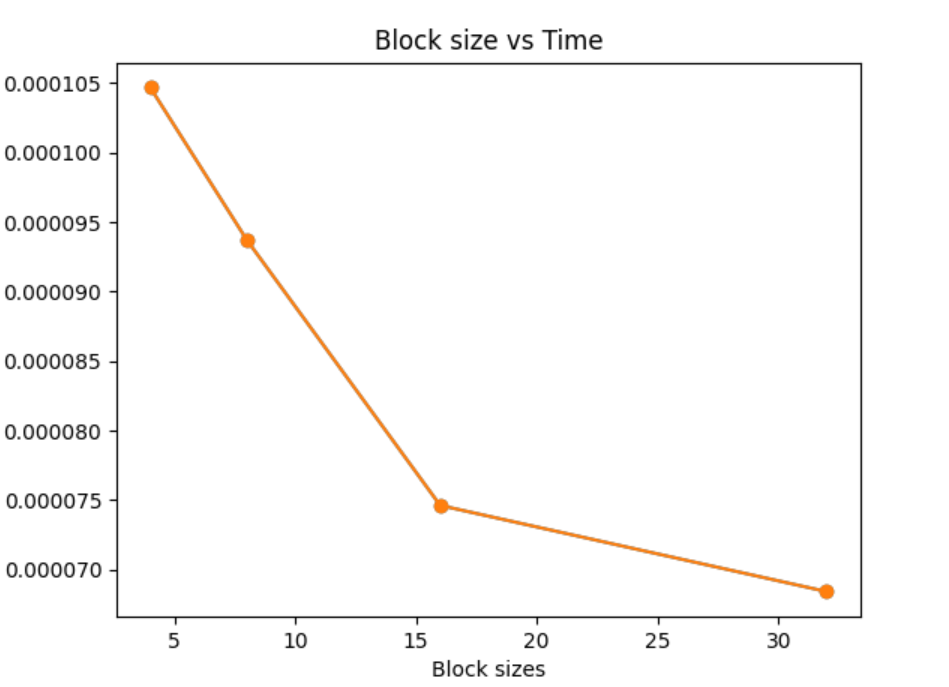
\includegraphics[width=1\linewidth]{GPU response time.png}
    \caption{Result photo}
    \label{fig:placeholder}
\end{figure}
\\In the first run, the response time was significantly longer than that of the CPU, but from the second run onward, it reduced drastically. This shows that for small tasks, GPU may take longer than CPU since the process involves several copy steps. GPU may only benefit in repetitive runs. In addition, the larger the number of block size, the shorter the response time for the GPU. 

\end{document}
